\section{Results}
The tool we built allows election officials to perform a general audit after an election.  Expanding these automated post-election analyses becomes particularly critical in those instances where the time between elections is short, as is typical in run-off elections.  This section discusses our findings after running our algorithms on various South Carolina elections.  The iVotronic files used for testing our analyses were downloaded from the website titled \textquotedblleft South Carolina Voting Information.\textquotedblright \footnote{www.scvotinginfo.com}

\subsection{Missing Votes}
Table~\ref{tab:pebs} summarizes the PEBs not uploaded during the General 2010 elections in South Carolina. The system file (EL68a) was used to identify which PEBs containing votes were not uploaded to the election reporting software. If the South Carolina counties had access to our tool during their canvass audits they could have quickly located those PEBs.

\begin{table*}
    \begin{center}
    \begin{tabular}{| c | c | c | c |}
    \hline                   
    County &PEBs used to collect votes &PEBs not uploaded &Votes not uploaded\\
    \hline
    Anderson &77 &1 &163\\
    \hline
    Colleton &36 &1 &122\\
    \hline
    Georgetown &36 &1 &92\\
    \hline
    Greenville &154 &3 &500\\
    \hline
    Horry &121 &2 &189\\
    \hline
    Richland &128 &5 &648\\
    \hline
    Sumter &60 &2 &368\\
    \hline
    \end{tabular}
    \end{center}
    \caption{PEBs not uploaded}
    \label{tab:pebs}
\end{table*}

The tool we implemented has reported a few instances of machines not being closed.  There was a single machine that wasn't closed in each of the following counties: Greenville County, Horry County, and Sumter County.  These are only detected if they are closed when the CF card is still in the machine and the complete audit data, including the closure event, is saved to the CF card.  If the audit data is not complete, we cannot determine whether a machine was closed or not.  There may be other cases that are undetectable by our analysis because a machine's audit data will not be in the event log or ballot image file if it has not been closed in the normal circumstances.

\subsection{Incomplete Audit Data}
There were a number of counties' audit logs from the South Carolina 2010 elections that showed incomplete data.  Our analysis detected six counties that did not have the same set of machines in both the event log and ballot images file.  Florence County had the most inconsistencies with 65 machines that had votes cast on them according to the event log, but no ballot images.  We also saw cases where there were ballot images for votes cast on machines that did not record any events on the event log.  We also found a couple of very odd situations, such as in Sumter County, where there were two machines that were flagged; one of these machines was in the event log, but not in the ballot image file, and the other machine was in the ballot images, but not in the event log.  In addition to an unusually large amount of missing data, the analysis of Florence county showed machines in both files that did not have the same number of votes cast as ballot images.  If election officials find this error when running an analysis,  they should re-upload the audit data to ensure a set of complete files.

\subsection{Polling Location Related Findings}

Figure~\ref{fig:late} is a histogram of the polling locations that closed late in Berkeley County.

\begin{figure}[h!]
  \caption{Polling locations that closed late in Berkeley County}
  \label{fig:late}
  \centering
    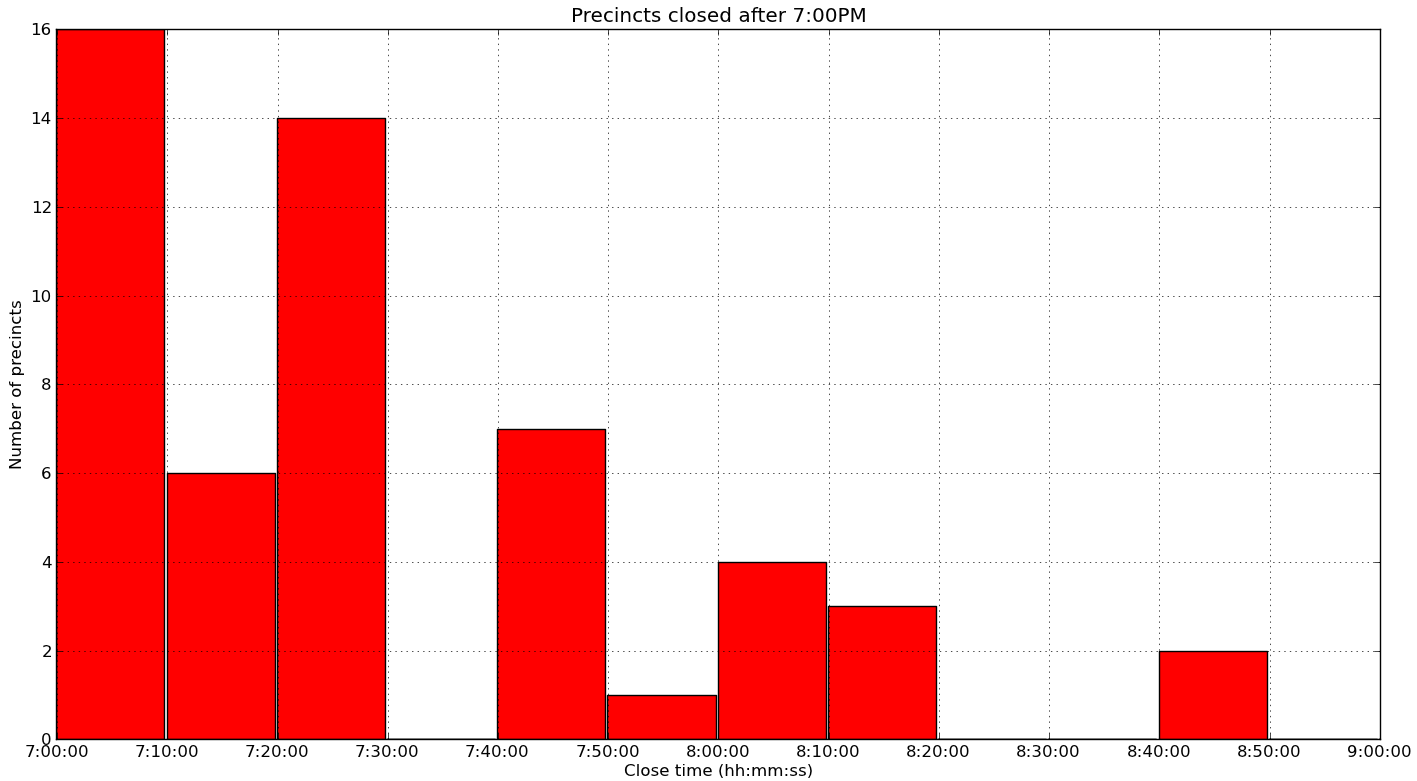
\includegraphics[width=0.5\textwidth]{berkeley}
\end{figure}

Table~\ref{tab:line} summarizes the times periods when the Berkeley County polling locations experienced long lines before 7 P.M.  In South Carolina polls close at 7 P.M.

\begin{table*}
    \begin{center}
    \begin{tabular}{| c | p{5cm} | p{4.5cm} |}
    \hline                   
    \# Precinct & Possibly not long lines experienced &Possibly long lines experienced\\
    \hline
    26 Huger&9:00 a.m. - 10:00 a.m. &7:00 a.m. - 9:00 a.m.\\
            &12:00 p.m. - 1:00 p.m. &10:00 a.m. - 12:00 m.\\
            &4:00 p.m. - 5:00 p.m. &1:00 p.m. - 4:00 p.m.\\
            &6:00 p.m. - 7:00 p.m. &5:00 p.m. - 6:00 p.m.\\
    \hline
    10 Cordesville &7:00 a.m. - 8:00 a.m.&8:00 a.m. - 12:00 m.\\
                   &12:00 m. - 1:00 p.m.&1:00 p.m. - 7:00 p.m.\\
    \hline  
    24 Hilton Cross Rd &12:00 m. - 1:00 p.m. &7:00 a.m. - 12:00 m.\\
                       &5:00 p.m. - 6:00 p.m. &1:00 p.m. - 7:00 p.m.\\
    \hline
    22 Hanahan 3 &7:00 a.m. - 5:00 p.m. &5:00 p.m. - 6:00 p.m.\\
                 &6:00 p.m. - 7:00 p.m.&\\
    \hline
    20 Hanahan 1 &12:00 m. - 1:00 p.m. &7:00 a.m. - 12:00 m.\\
                 &2:00 p.m. - 3:00 p.m. &1:00 p.m. - 2:00 p.m.\\
                 &5:00 p.m. - 6:00 p.m. &3:00 p.m. - 5:00 p.m.\\
                 &                      &6:00 p.m. - 7:00 p.m.\\
    \hline
    \end{tabular}
    \end{center}
    \caption{Long Lines in Berkeley County}
    \label{tab:line}
\end{table*}




\subsection{Hardware Issues}
The machines used in South Carolina have experienced frequent potential hardware issues.  For example, the combination of machines in Berkeley County experienced votes cast on a machine when the machine was not calibrated, machines with possible low batteries, and at least one machine that closed early.  Our analysis found that there were seven counties where at least one machine was possibly not calibrated when votes were cast on that machine; these errors spanned 12 different polling locations.  We suggest an election official or technician inspect these machines for possible calibration issues.  We had similar findings when searching for terminals that recorded a "Warning - Terminal Closed Early" event.  There were machines with this warning in seven counties and 13 polling locations.  Terminals should not close before 7 P.M. in South Carolina on election day; for this reason, we recommend that these machines be evaluated for potential problems that would have caused early closure.  When our tool reports machines with power supply issues and possibly low batteries, election officials should verify that the machine is working properly and does not need maintenance.  Florence County and Greenville county experienced a number of Internal Power Supply - related events; at least one machine in each precinct had 53 and 63 instances of this event, respectively.  This could be a possible indicator that the battery is running low; therefore, the election officials should take action to ensure all machines work properly in future elections.

\subsection{Procedural Errors}
Our findings reveal the improvements needed for poll worker training and for various procedures.  When opening and closing a machine, the same master PEB should be used, but in 11 counties there were cases of opening and closing machines with different PEBs.  Our results showed a correlation between this error and certain precincts, where poll workers made those mistakes repeatedly.  Colleton County had five instances of this procedural error, but four of those instances took place at one polling location; Walterboro No 4 had machines 5129946, 5133679, 5138439, and 5138563 opened with PEB 155914, but closed with PEB 155925.  This should raise a red flag to the election officials that they may need to emphasize the correct procedure in poll worker training.  When poll workers activate ballots for voters, they should do so with a non-master PEB; we saw two counties that had an unusually high number of violations of this procedure.  Horry County and Richland County had 22 and 32 instances of this violation, respectively.  When election officials see this result, they may wish to revise poll worker training.  Our tool also analyzes the reasons why votes were canceled, which could give insight to procedural errors.  There is likely to be a certain number of vote cancellations due to a number of reasons, but our tool will only report the machines that recorded an abnormally large amount of vote cancellations for a specific reason.  Colleton County had a machine that recorded 12 instances of vote cancellations due to a terminal problem; in this case, we would recommend the officials to inspect the machine for potential hardware problems.  A machine in Lexington County experienced an unusually large number of vote cancellations due to a "wrong ballot"; this could be the result of many problems.  The machine may have a calibration issue, or there may be a procedural error in that the poll workers are repeatedly selecting the wrong ballot.

\subsection{Date/Time Errors}
